\begin{enumerate}[label=\thechapter.\arabic*,ref=\thechapter.\theenumi]
\numberwithin{equation}{enumi}
\numberwithin{figure}{enumi}
\numberwithin{table}{enumi}
\item Cauchy's Theorem: \label{Cauchy} \\
From Figure \ref{fig:fig1_Cauchy}
\begin{align}
    \int_C f\brak{z}dz &= \int_{Cr} f\brak{z}dz
\end{align}
\begin{figure}[ht]
    \centering
    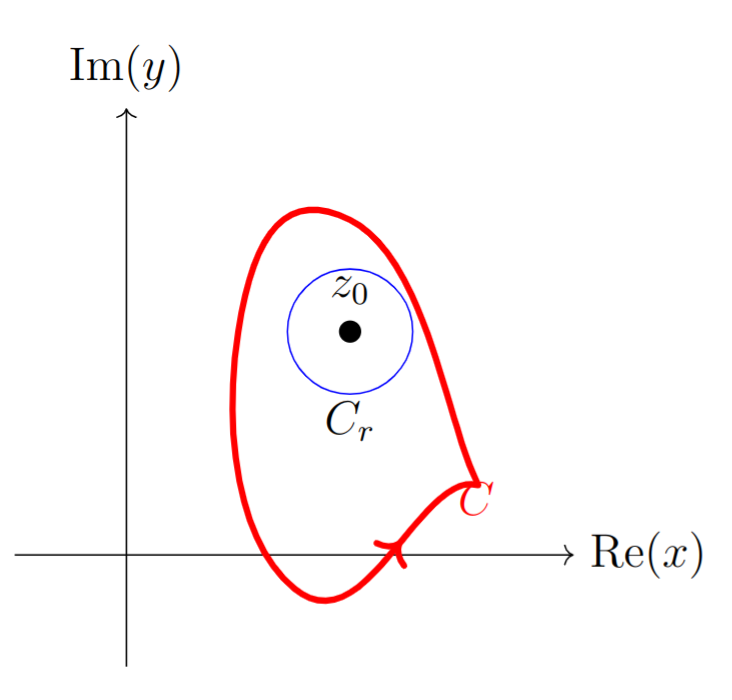
\includegraphics[width=0.5\textwidth]{app/figs/img1.png}
    \caption{Figure1}
    \label{fig:fig1_Cauchy}
\end{figure}
Since  $g\brak{z}$ is continuous we know that $\abs{g\brak{z}}$ is bounded inside  $C_r$. Say,  $\abs{g\brak{z}}<M$. The corollary to the triangle inequality says that
\begin{align}
    \abs{\int_{C_r}f\brak{z}\, dz} &\leq M2\pi r.
\end{align}
Since  $r$ can be as small as we want, this implies that
\begin{align}
    \int_{Cr} f\brak{z}dz &= 0
\end{align}
let \begin{align}
    g\brak{z} &= \frac{f\brak{z} - f\brak{z_0}}{z-z_0}\\
    \lim_{z \to z_0} g(z) &= f'(z_0)\\
    \int_{C} g(z)\ dz = 0, &\implies \int_C \frac{f(z) - f(z_0)}{z - z_0} \ dz = 0
\end{align}
Thus,
\begin{align}
    \int_{C} \frac{f(z)}{z - z_0}\ dz = \int_C \dfrac{f(z_0)}{z - z_0}\ dz = 2\pi i f(z_0) \label{eq:eq3_gate_2022_ma_14}
\end{align}

Using Cauchy's Theorem,
\begin{align}
    \int_C f\brak{z} &= 0\\
    f\brak{a} &= \frac{1}{2 \pi i}\oint_C\frac{f\brak{z}}{z-a}\, dz\\
    f^{n}\brak{a} &= \frac{n!}{2 \pi i}\oint_C\frac{f\brak{z}}{\brak{z-a}^{n+1}}\, dz
\end{align}
\pagebreak
\item Residue Theorem:\label{Residue} \\
From eq (\ref{eq:eq3_gate_2022_ma_14})
\begin{align}
    \int_C f\brak{z}\, dz &= 2 \pi i \sum{Res \, f\brak{a}} \label{eq:eq1_gate_ma_2022_14_054}
\end{align}
where, for n repeated poles,
\begin{align}
    Res \, f\brak{a} &= \lim_{z \to a}\frac{1}{\brak{n-1}!}\brak{\frac{d^{n-1}}{dz^{n-1}}\sbrak{\brak{z-a}^n\, f\brak{z}}} \label{eq:eq2_gate_ma_2022_14_054}
\end{align}
\end{enumerate}
